\section{Optical SM and SMP modulation techniques}
\label{sec:osm}

\graphicspath{{_MIMOSpace/figures_osm/}}

%\subsection{SM and SMP system outline}
%\label{subsec:osmSystem}

\begin{figure}[t]
	\centering
		\begin{subfigure}{0.49\textwidth}
		\centering
				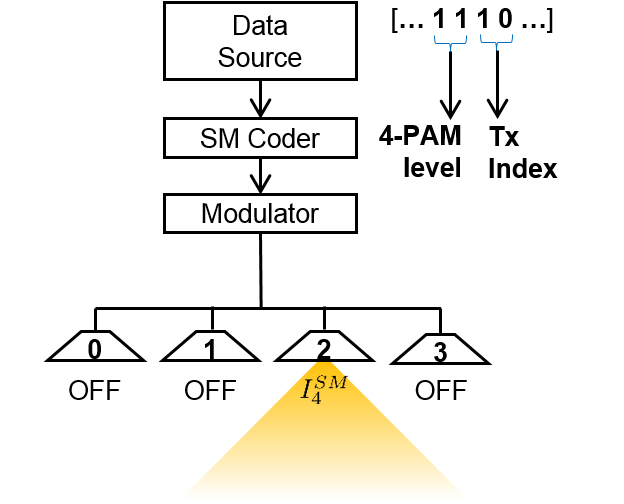
\includegraphics[trim=0in 0in 0in 0in, clip=false, width=2.5in]{figSM.png}
		\caption{}
		\label{figSM}			
		\end{subfigure}
		\hfill
		\begin{subfigure}{0.49\textwidth}
		\centering
				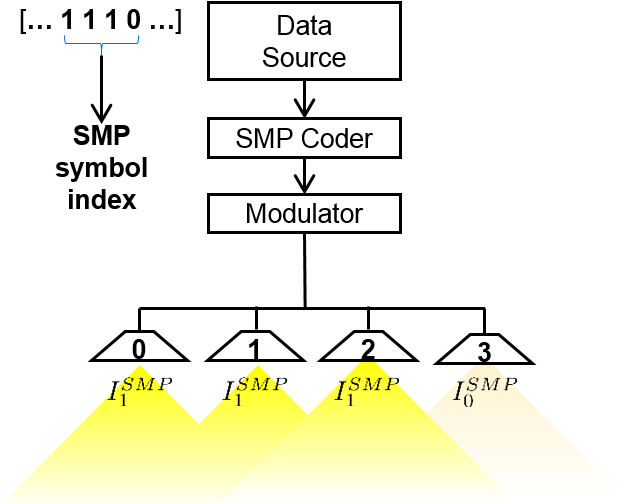
\includegraphics[trim=0in 0in 0in 0in, clip=false, width=2.5in]{figSMP.png}
				\caption{}
				\label{figSMP}
		\end{subfigure}
\caption[SM and SMP implementation block diagram]{SM and SMP implementation block diagram for 4 bits/symbol (a) SM implementation with $N_{\text{tx}} = 4$ and $M = 4$ (b) SMP implementation with $N_{\text{tx}} = 4$ and $M = 2$}
	\label{fig:SpatialModulation}
\end{figure}

Optical SM was introduced in \cite{mes06a} as a low complexity modulation technique that enhances spectral efficiency by exploiting spatial dimension. SM encodes $k =$ log$^{ }_{2}(N_{\text{tx}})$ bits in the transmitter index in addition to $m=$ log$^{ }_{2}(M)$ bits using $M$-ary modulation. Thus SM transmits $r=k+m=$ log$^{ }_{2}(MN_{\text{tx}})$ bits per SM symbol. The encoded information stream is divided into $r$ bits long contiguous segments. First $m$ bits of each symbol are mapped to one of the $M$-ary constellation points while the last $k$ bits of each symbol select the luminaire that transmits the selected constellation point. SM implementation is illustrated in \figurename{ \ref{figSM}} for $N_{\text{tx}}=4$ transmitters and 4-PAM. $M$-PAM intensity levels for SM are selected as in (\ref{eqSMPAM}) where $P^{\text{tx}}_{\text{avg}}$ is the average signal constraint to maintain desired illumination. Given a bit sequence forming a symbol [1 1 1 0], PAM level 3 $(I_4^{\text{SM}})$ is radiated using transmitter index $2$.

\begin{equation}
	\label{eqSMPAM}
	P_{x}^{\text{SM}} = \frac{2P^{\text{tx}}_{\text{avg}}}{M+1}x; 1 \leq x \leq M
\end{equation}

On the other hand, SMP uses $M$-ary modulation for each luminaire to transmit information. SMP with $N_{\text{tx}}$ number of luminaires jointly generates $M^{N_{\text{tx}}}$ unique symbols. Each SMP symbol transmits $r=N_{\text{tx}}$ log$^{ }_{2}(M)$ bits. Each $r$ bit long section of encoded information stream is then mapped to one of the $M^{N_{\text{tx}}}$ unique symbols. SMP for a setup with $N_{\text{tx}}=4$ transmitters and 2-PAM is illustrated in \figurename{ \ref{figSMP}}. $M$-PAM intensity levels for SMP are selected as in (\ref{eqSMPPAM}) where $P^{\text{tx}}_{\text{avg}}$ is the average signal constraint to maintain desired illumination. A bit sequence forming a symbol [1 1 1 0] is jointly mapped to the $15^{\text{th}}$ out of $N_{\text{tx}}$log$^{ }_{2}(M)=16$ possible unique symbols.
\begin{equation}
	\label{eqSMPPAM}
	P_{x}^{\text{SMP}} = \frac{2P^{\text{tx}}_{\text{avg}}}{M-1}x; 0\leq x < M
\end{equation}

For a channel with equally likely symbols, a maximum likelihood (ML) detector is the optimal detector. If noise is AWGN, this reduces to nearest neighbor (NN) detection. Having observed ${\bf{Y}}$ and knowing ${\bf{H}}$, estimated symbol $\hat{{\bf{X}}}$ is the symbol closest to observation ${\bf{Y}}$ in Euclidean space. The signal detection can be written as
\begin{gather}
\begin{aligned}
	\hat{{\bf{X}}} =&{} \argmax_{\forall{\bf{X_i}}} p_{{\bf{Y}}|{\bf{X}}}({\bf{Y}}|{\bf{X_i}},{\bf{H}})\\
	=&{} \argmin_{\forall{\bf{X_i}}} ||{\bf{Y}}-{\bf{H}}{\bf{X_i}}||_{F}
\label{eq:ML}
\end{aligned}
\end{gather}
where ${\bf{X_i}}$ are the different symbols and $||.||_{F}$ is the Frobenius norm.

In an indoor VLC system, luminaires need to maintain an average emitted radiant flux over different overlapping time windows so that the perceived illumination remains constant. Thus a fair performance comparison between different modulation schemes can be made when they emit the same radiant flux. Thus the SNR is defined as
\begin{equation}
  \label{eqOSMSNRTX}
	\text{SNR} = \frac{(\text{e}P_{\text{avg}}^{\text{tx}})^2}{\sigma_{\text{n}}^2}
\end{equation}
where $P_{\text{avg}}^{\text{tx}}$ is the average radiant flux emitted by a transmitter, e is the optical to electrical conversion factor (AW$^{-1}\Omega^{-2})$ and $\sigma_{\text{n}}^2$ is the noise power. Without loss of generality, e = 1 is assumed. This SNR definition is used in reference \cite{fat13a} and thus used here to demonstrate performance enhancement of SM and SMP systems with imaging receiver when compared to non--imaging receiver considered in the reference.
%%%%%%%%%%%%%%%%%%%%%%%%%%%%%%%%%%%%%%%%%%%%%%%%%%%%%%%%%%%%%%%%
%%%%%%%%%%%%%%%%%%%%%%%%%%%% RESULTS %%%%%%%%%%%%%%%%%%%%%%%%%%%
%%%%%%%%%%%%%%%%%%%%%%%%%%%%%%%%%%%%%%%%%%%%%%%%%%%%%%%%%%%%%%%%

\section{SM and SMP system performance with imaging receiver}
\label{sec:osmAnalysis}
% DELETED ON 11 MARCH 2015
%An example system is considered which has 4 transmitters arranged on a regular grid with pitch $P_{\text{tx}}$. Each transmitter has side length $\alpha_{\text{tx}}^{min}$ and diagonal $\alpha_{\text{tx}}^{max}$. The imaging receiver optics has focal length $f$. Sensor is made of large enough contiguous PD array such that all the 4 transmitter images (spots) fall on the sensor for all the different analysis configurations. Each PD is assumed to have a square shape with side length $\alpha_{\text{px}}^{min}$ and diagonal $\alpha_{\text{px}}^{max}$. The receiver surface is assumed parallel to the transmitter plane. Receiver at a distance $d$ from the transmitter plane sees a magnification $M=f/(d-f)$. If $d>>f$, which is true is most practical scenarios, $M\approx f/d$. 

The effects of varying transmitter array and imaging receiver configurations on the BER performance of SM and SMP systems are studied. An array of $N_{\text{tx}} = 4$ transmitters that are arranged on a regular grid with pitch $P_{\text{tx}}$ is considered. To achieve 4 bits/sym, SM with $N_{\text{tx}}=4$ and $M=4$-PAM and SMP with $N_{\text{tx}}=4$ and $M=2$-PAM are implemented. To achieve 8 bits/sym, SM with $N_{\text{tx}}=4$ and $M=64$-PAM and SMP with $N_{\text{tx}}=4$ and $M=4$-PAM are implemented. The vertical distance $||\vm{d}^{z}_{j}||$ between the transmitter and receiver planes is 2 m. Lambertian luminaires of order 1 are assumed to have a spectral power distribution that is approximated by a sum of Gaussians as in \cite{gru08b}. The effective responsivity of each pixel is equal to 0.4 A/W. Within this context, it is assumed that the pixel grid is large enough to ensure that each of the four spots fall on the sensor for each of the different configurations considered below.

Using the parameters specified above, the channel gains are of the order of $10^{-7}$ for all configurations. Thus the transmitted signal power is about $140$ dB higher than the received signal power. Typically, the SNR is defined as the ratio of received signal power to noise power. However, given SNR as defined in Eq. \eqref{eqOSMSNRTX}, there is an offset of at least +140 dB over typical definition.

%%%%%%%%%%%%%%%%%%%%%%%%%%%%%%%%%%%%%%%%%%%
%%%%%%%%%%%%%%%%% COMPARE %%%%%%%%%%%%%%%%%
%%%%%%%%%%%%%%%%%%%%%%%%%%%%%%%%%%%%%%%%%%%
\subsubsection{Imaging vs non--imaging receiver}
\label{subsubsec:osmResultsCompare}
Performance gains of using an imaging receiver over a non--imaging receiver are analyzed in this subsection. The transmitter and modulation parameters are the same as described above. For this analysis, $P_{\text{tx}}=$ 0.5 m is considered. The non--imaging receiver is made up of $2\times2$ array of pixels; each with a side length of 1 mm and a pitch of 1 mm. Each pixel has a concentrator of refractive index $1.5$ and FOV of 60 $\deg$. For the imaging receiver, the sensor is modeled as $2\times2$ array of pixels with side length and pitch of 1 mm. The imaging lens is defined to have sufficient magnification to align the images of the four transmitters each with four pixels respectively. 
\afterpage{%
	\clearpage
\begin{figure}
	\centering
		\begin{subfigure}{\textwidth}
			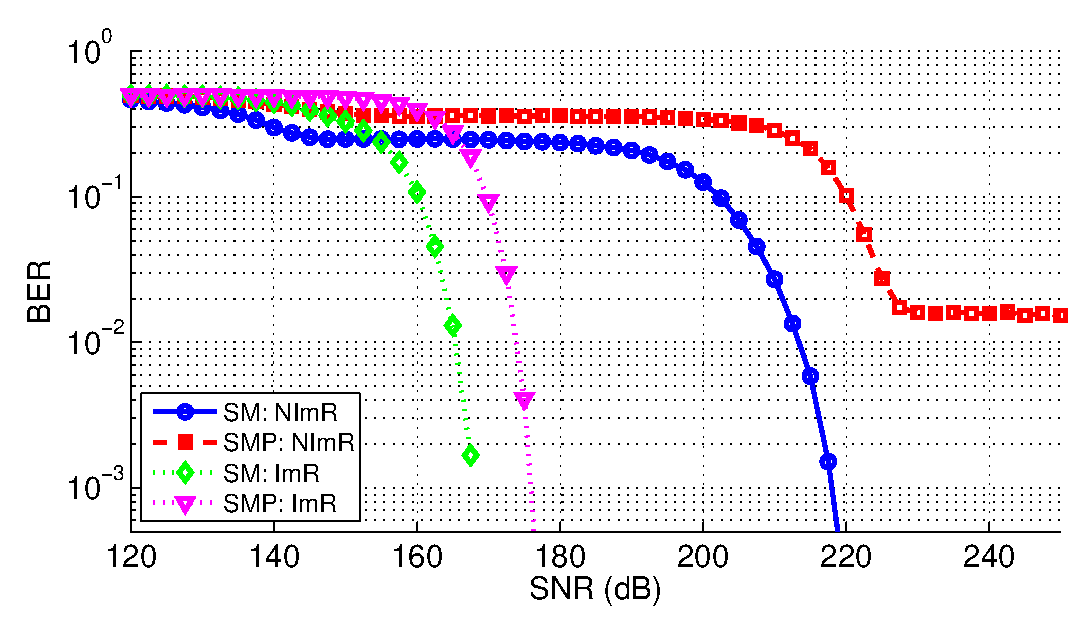
\includegraphics[width=0.9\textwidth]{figCompare4B.eps}
			\caption{4 bits/sym}
			\label{figCompare4B}
		\end{subfigure}
	  \vfill
		\begin{subfigure}{\textwidth}
		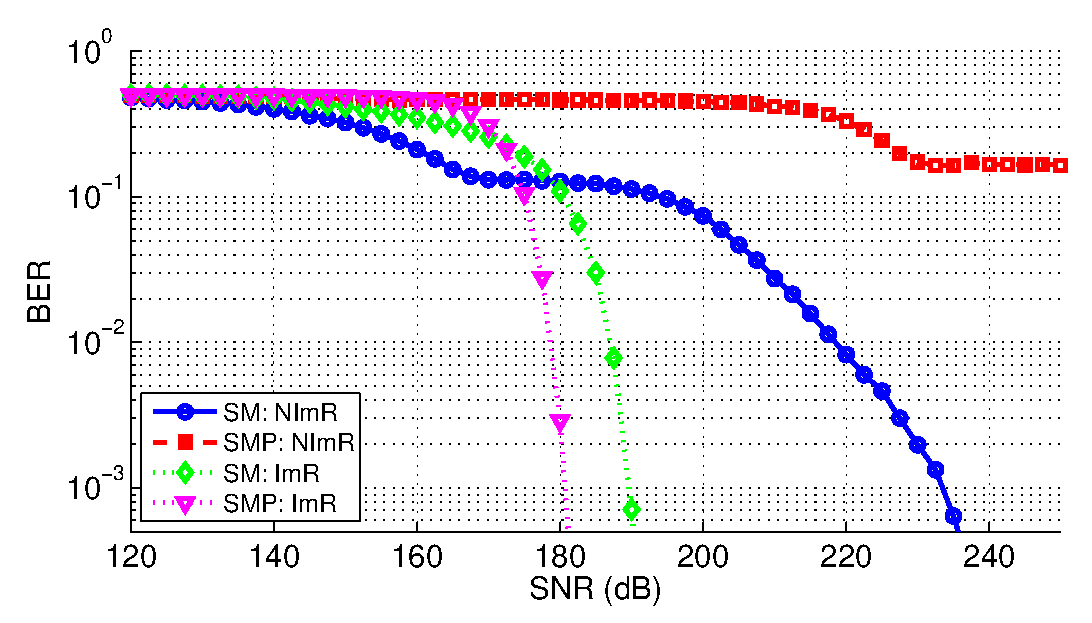
\includegraphics[width=0.9\textwidth]{figCompare8B.eps}
		\caption{8 bits/sym}
		\label{figCompare8B}
		\end{subfigure}
	
	\caption[SM and SMP performance comparison]{Performance comparison of SM and SMP using non--imaging (NImR) and imaging (ImR) receiver}
	\label{figCompare}
\end{figure}
\clearpage% Flush page
}
The FOV of the receiver changes with the sensor dimensions. The maximum FOV is defined as 60 $\deg$; the same as in non--imaging receiver case. A fair performance comparison between the two receiver configurations can be made under the assumption that the same average signal radiant flux is incident on both. Thus, the aperture of the imaging receiver is modeled to have an area of  1 mm$^{2}$.

BER vs SNR curves for SM and SMP using non--imaging receiver and imaging receiver are shown in \figurename{ \ref{figCompare}}. At low average signal powers, using a non--imaging receiver, shot noise is the dominant source of noise. At high signal powers, ICI dominates the noise for the non--imaging receiver because the channel matrix coefficients are highly correlated \cite{zen09a}. This can be seen as two regions of the BER curves when using a non--imaging receiver. SM mitigates ICI and is thus more robust as compared to SMP in this scenario. BER achieved by SMP with non--imaging receiver are greater than $10^{-3}$ for the range of SNR considered and thus cannot be improved by forward error correction (FEC). SM needs a high transmit signal power to achieve BER $\leq 10^{-3}$ for both 4 and 8 bits/sym. Conversely, imaging receiver completely demultiplexes the four transmit signals while generating a diagonal channel matrix and thus avoids ICI under ideal setup. To achieve BER $=10^{-3}$ at 4 bits/sym, SM with imaging receiver performs about 8 dB better that SMP with imaging receiver and about 45 dB better than SM with non--imaging receiver. SMP packs more bits spatially in transmitter location as compared to SM. Thus, to achieve higher spectral efficiency while keeping the number of transmitters the same, more $M$-ary PAM levels are needed for SM as compared to SMP thus quickly degrading SM's performance. To achieve BER $=10^{-3}$ at 8 bits/sym, SMP with imaging receiver outperforms SM with imaging receiver by about 10 dB and SM with non--imaging receiver by about 52 dB. The channel matrix coefficient decorrelation afforded by imaging receiver provide huge SNR gains over non--imaging receiver for a given BER.

%%%%%%%%%%%%%%%%%%%%%%%%%%%%%%%%%%%%%%%%%%%%
%%%%%%%%%%%%%%%%%%% ALPHA %%%%%%%%%%%%%%%%%%
%%%%%%%%%%%%%%%%%%%%%%%%%%%%%%%%%%%%%%%%%%%%

\subsubsection{Varying $\alpha_{\text{s}}$}
\label{subsec:osmResultsAlpha}

\begin{figure}[!t]
	\centering
		\begin{subfigure}{0.49\textwidth}
			\centering
			\includegraphics[width=0.63\textwidth]{figASspN4A05.eps}
			\label{figASspN4A05}
		\caption{$\alpha_{\text{s}}=0.5$}
		\end{subfigure}
		\hfill
		\begin{subfigure}{0.49\textwidth}
			\centering
			\includegraphics[width=0.63\textwidth]{figASspN4A1.eps}
			\label{figASspN4A1}
		\caption{$\alpha_{\text{s}}=1.0$}
		\end{subfigure}
		\vfill
		\begin{subfigure}{0.49\textwidth}
			\centering
			\includegraphics[width=0.63\textwidth]{figASspN4A14.eps}
			\label{figASspN4A14}
		\caption{$\alpha_{\text{s}}=1.41$}
		\end{subfigure}
		\hfill
		\begin{subfigure}{0.49\textwidth}
			\centering
			\includegraphics[width=0.63\textwidth]{figASspN4A2.eps}
			\label{figASspN4A2}
		\caption{$\alpha_{\text{s}}=2.0$}
		\end{subfigure}
	\caption{Spots on the sensor for different $\alpha_{\text{s}}$}
	\label{figASSpots}
\end{figure}

\afterpage{%
	%\clearpage
\begin{figure}
	\centering
		\begin{subfigure}{\textwidth}
			\centering
			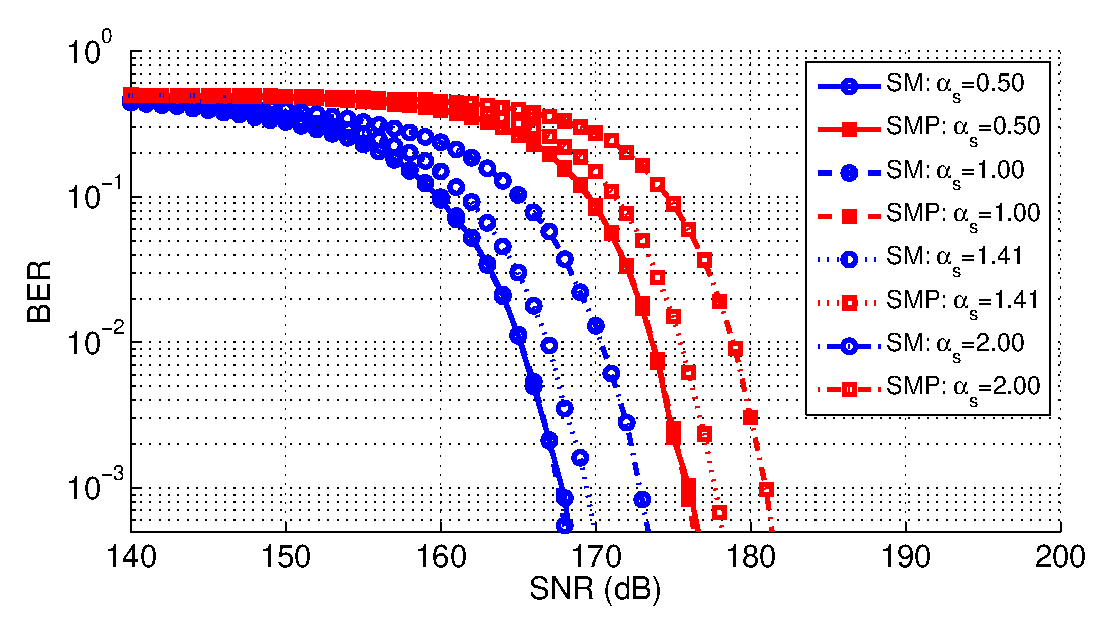
\includegraphics[width=0.9\textwidth]{figASN4B4.eps}
			\caption{4 bits/sym}
			\label{figASN4B4}
		\end{subfigure}
		
		\begin{subfigure}{\textwidth}
			\centering
			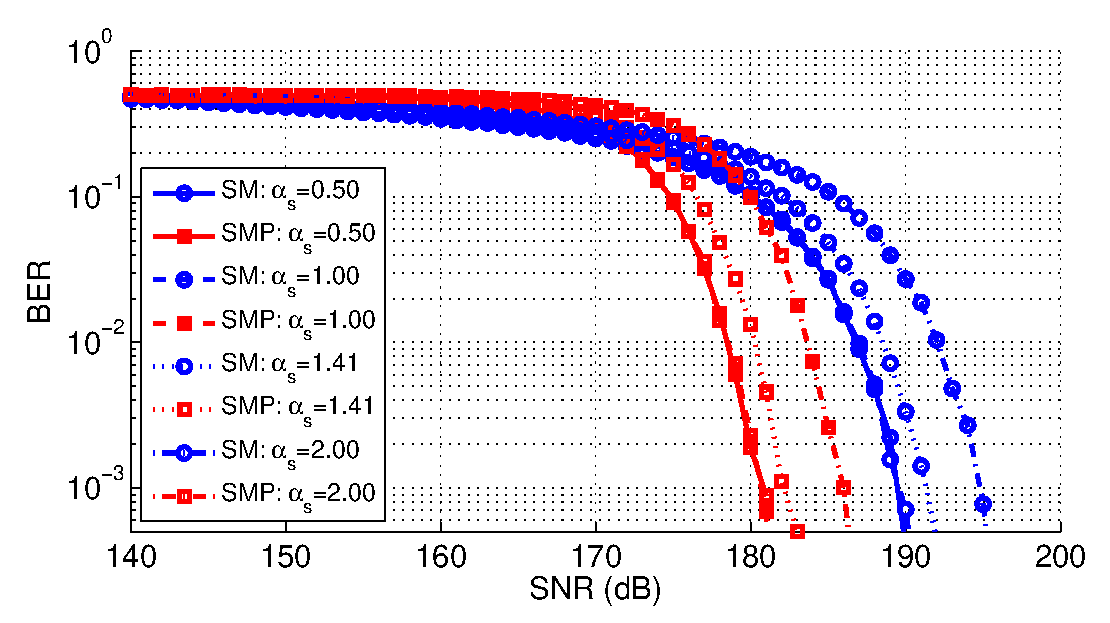
\includegraphics[width=0.9\textwidth]{figASN4B8.eps}
			\caption{8 bits/sym}
			\label{figASN4B8}
		\end{subfigure}
		
		\caption{BER vs SNR for different $\alpha_{\text{s}}$}
		\label{figASBvS}
\end{figure}
	%\clearpage% Flush page
}

For this analysis, $\alpha_{\text{s}}$ is varied while keeping $\delta_{\text{s}}$ and $\mu_{\text{s}}$ fixed. As illustrated in \figurename{ \ref{figASSpots}}, $\alpha_{\text{s}}$ affects only the spot size. As $\alpha_{\text{s}}$ increases, spots on the sensor overlap increasingly more number of pixels degrading the BER performance. Increasing the number of pixels per spot also increases the noise for each link thus causing the drop in performance. Very small pixel sizes or very large transmitter sizes also cause increase in $\alpha_{\text{s}}$. A smaller pixel size does enable the system to pack more channels provided $\alpha_{\text{s}}$ is relatively small. On the other hand, having very small pixel sizes or alternately large transmitter illumination surface tend to increase $\alpha_{\text{s}}$ and force the system to operate in a suboptimal configuration.

BER vs SNR curves for SM and SMP for different values of $\alpha_{\text{s}}$ are shown in \figurename{ \ref{figASBvS}}. To achieve BER $\leq10^{-3}$ at 4 bits/sym, SNRs of about [168, 168, 170, 173] dB and [176, 176, 178, 181] dB are needed for $\alpha_{\text{s}}$ = [0.5, 1, 1.41, 2]  with SM and SMP respectively. To achieve BER $\leq10^{-3}$ at 8 bits/sym, SNRs of about [190, 190, 192, 195] dB and [181, 181, 183, 186] dB are needed for $\alpha_{\text{s}}$ = [0.5, 1, 1.41, 2] with SM and SMP respectively. Thus there is about a 2 dB SNR penalty for system operating at $\alpha_{\text{s}}=1.41$ and 5 dB SNR penalty for system operating at $\alpha_{\text{s}}=2$ as compared to that at $\alpha_{\text{s}}=1$.

%%%%%%%%%%%%%%%%%%%%%%%%%%%%%%%%%%%%%%%%%%
%%%%%%%%%%%%%%%%%%% ETA %%%%%%%%%%%%%%%%%%
%%%%%%%%%%%%%%%%%%%%%%%%%%%%%%%%%%%%%%%%%%
\subsubsection{Varying $\eta_{\text{s}}$}
\label{subsubsec:osmResultsEta}
\begin{figure}[!t]
	\centering
		\begin{subfigure}{0.49\textwidth}
			\centering
			\includegraphics[width=0.63\textwidth]{figESspN4E0.eps}
			\caption{$\eta_{\text{s}}=0$}
			\label{figESspN4E0}
		\end{subfigure}
		\hfill
		\begin{subfigure}{0.49\textwidth}
			\centering
			\includegraphics[width=0.63\textwidth]{figESspN4E071.eps}
			\caption{$\eta_{\text{s}}=0.71$}
			\label{figESspN4E071}
		\end{subfigure}
		\vfill
		\begin{subfigure}{0.49\textwidth}
			\centering
			\includegraphics[width=0.63\textwidth]{figESspN4E1.eps}
			\caption{$\eta_{\text{s}}=1$}
			\label{figESspN4E1}
		\end{subfigure}
		\hfill
		\begin{subfigure}{0.49\textwidth}
			\centering
			\includegraphics[width=0.63\textwidth]{figESspN4E14.eps}
			\caption{$\eta_{\text{s}}=1.41$}
			\label{figESspN4E14}
		\end{subfigure}
		
		\caption{Spots on sensor for different $\eta_{\text{s}}$}
		\label{figESSpots}
\end{figure}

\afterpage{%
	%\clearpage
	\begin{figure}[!t]
		\centering
			\begin{subfigure}{\textwidth}
				\centering
				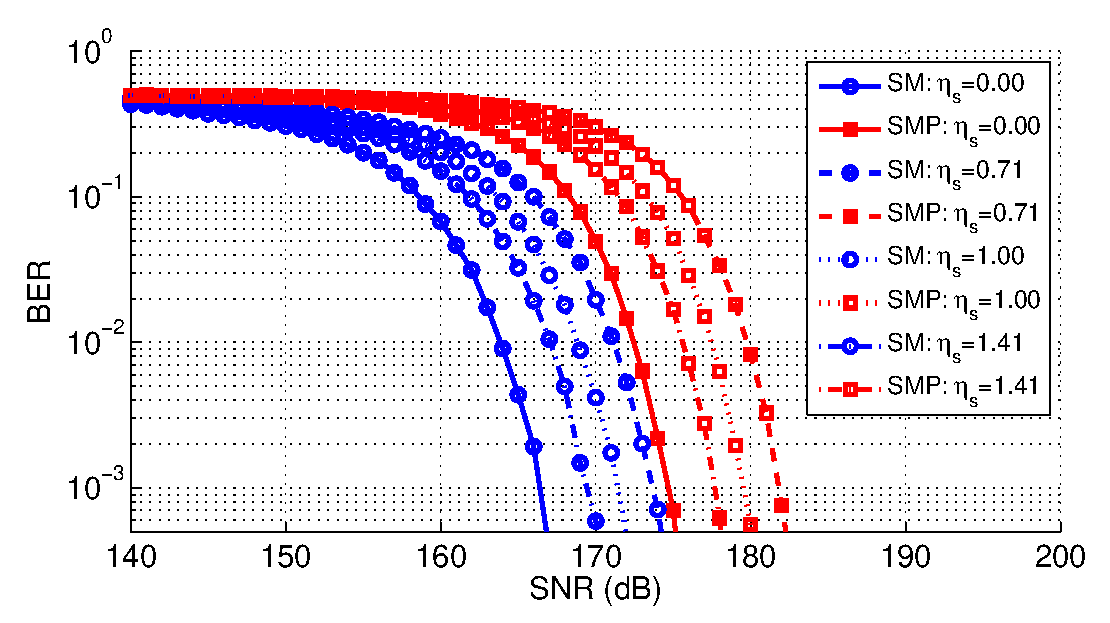
\includegraphics[width=0.9\textwidth]{figESN4B4.eps}
				\caption{4 bits/sym}
				\label{figESN4B4}
			\end{subfigure}
			\vfill
			\begin{subfigure}{\textwidth}
				\centering
				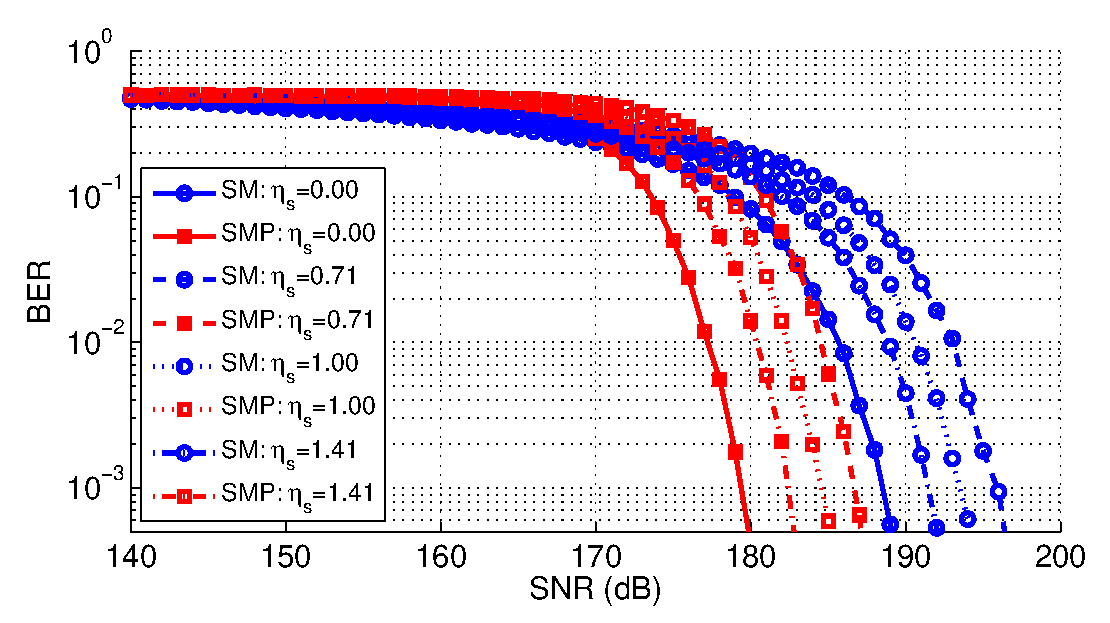
\includegraphics[width=0.9\textwidth]{figESN4B8.eps}
				\caption{8 bits/sym}
				\label{figESN4B8}
			\end{subfigure}
			
			\caption{BER vs SNR for different $\eta_{\text{s}}$.}
			\label{figESBvS}
	\end{figure}
	\clearpage% Flush page
}

For this analysis, $\eta_{\text{s}}$ (alternately $\delta_{\text{s}}$) is varied while keeping $\alpha_{\text{s}}$ and $\mu_{\text{s}}$ fixed. Thus only the effect of change in spot pitch affects the BER performance. As illustrated in \figurename{ \ref{figESSpots}}, as $\eta_{\text{s}}$ increases, distance between the spots on the sensor increases as they push further apart.

BER vs SNR curves for SM and SMP for different values of $\eta_{\text{s}}$ are shown in \figurename{ \ref{figESBvS}}. To achieve BER $\leq 10^{-3}$ at 4 bits/sym, SNRs of about [167, 174, 172, 170] dB and [175, 182, 180, 178] dB are needed for $\eta_{\text{s}}$ = [0, 0.71, 1, 1.41] with SM and SMP respectively. To achieve BER $\leq 10^{-3}$ at 8 bits/sym, SNRs of about [189, 196, 194, 192] dB and [180, 187, 185, 183] dB are needed for $\eta_{\text{s}}$ = [0, 0.71, 1, 1.41] with SM and SMP respectively. We see that the BER performance is best when the spot overlaps minimum number of pixels and worst when the spot is centered at a corner of a pixel thus maximizing the number of pixels it overlaps with. In this setup, for BER $=10^{-3}$, there is an SNR penalty of about 7 dB between the best and worst cases. The slight drop in performance for $\eta_{\text{s}}=1.4$ as compared to $\eta_{\text{s}}=0$ can be attributed to drop in free-space gain caused by the larger distance per link as a result of increased transmitter pitch.

%%%%%%%%%%%%%%%%%%%%%%%%%%%%%%%%%%%%%%%%
%%%%%%%%%%%%%%%%%% MU %%%%%%%%%%%%%%%%%%
%%%%%%%%%%%%%%%%%%%%%%%%%%%%%%%%%%%%%%%%
\subsubsection{Varying $\mu_{\text{s}}$}
\label{subsubsec:osmResultsMu}
In this analysis, $\mu_{\text{s}}$ is varied by varying focal length $f$. Alternately, it can be varied by changing length of optical axis $||\vm{d}^{z}_{j}||$. Varying $\mu_{\text{s}}$ affects both $\alpha_{\text{s}}$ and $\eta_{\text{s}}$ simultaneously. This captures their combined impact on the BER performance. We see from \figurename{ \ref{figMSSpots}} that increasing $\mu_{\text{s}}$ not only increases the spot size but also pushes the spots away from each other. Note unlike in previous case, the transmitter pitch remains constant ($P_{\text{tx}}>0$).

BER vs SNR curves for SM and SMP for different values of $\mu_{\text{s}}$ are shown in \figurename{ \ref{figMSBvS}}. To achieve BER $=10^{-3}$ at 4 bits/sym, SNRs of about [167, 173, 169, 173] dB and [175, 181, 177, 181]dB are needed for $\mu_{\text{s}}$ = [0.5, 1, 1.41, 2] with SM and SMP respectively. To achieve BER $=10^{-3}$ at 8 bits/sym, SNRs of about [189, 195, 191, 195] dB and [180, 186, 182, 186] dB are needed for $\mu_{\text{s}}$ = [0.5, 1, 1.41, 2] with SM and SMP respectively.

The best performance is obtained for $\mu_{\text{s}}\leq 0.5$. This is because at this value of $\mu_{\text{s}}$, $\alpha_{\text{s}}<1$ and $\eta_{\text{s}}$ is such that all spots lie on different adjacent pixels. It can also be inferred that given enough transmitters in the room, at $\mu=0.5$, every single pixel could get signal from a single transmitter thus greatly improving the capacity of the channel. 
%If the luminaires transmit with different power levels or if the channels gains are significantly different, capacity maximizing $\mu_{\text{s}}$ is an optimization problem to be solved.

\begin{figure}[!t]
	\centering
		\begin{subfigure}{0.49\textwidth}
			\centering
			\includegraphics[width=0.63\textwidth]{figMSspN4M05.eps}
			\caption{$\mu_{\text{s}}=0.5$}
			\label{figMSspN4M05}
		\end{subfigure}
		\hfill
		\begin{subfigure}{0.49\textwidth}
			\centering
			\includegraphics[width=0.63\textwidth]{figMSspN4M1.eps}
			\caption{$\mu_{\text{s}}=1$}
			\label{figMSspN4M1}
		\end{subfigure}
		\vfill
		\begin{subfigure}{0.49\textwidth}
			\centering
			\includegraphics[width=0.63\textwidth]{figMSspN4M14.eps}
			\caption{$\mu_{\text{s}}=1.41$}
			\label{figMSspN4M14}
		\end{subfigure}
		\hfill
		\begin{subfigure}{0.49\textwidth}
			\centering
		\includegraphics[width=0.63\textwidth]{figMSspN4M2.eps}
			\caption{$\mu_{\text{s}}=2$}
			\label{figMSspN4M2}
		\end{subfigure}
		\caption{Spots on sensor for different $\mu_{\text{s}}$}
		\label{figMSSpots}
\end{figure}

At lower bit rates, SM benefits from having higher transmit power per symbol at lower $M$-PAM level. To achieve higher bit-rates, higher $M$-PAM levels push the constellations closer to each other thus quickly degrade the SM performance as compared to SMP. As shown in \figurename{ \ref{figASBvS}}, \figurename{ \ref{figESBvS}} and \figurename{ \ref{figMSBvS}}, to achieve BER $=10^{-3}$, at 4 bits/sym, SM performs 8-10 dB better while at 8 bits/sym, SMP performs 8-10 dB better.

%\afterpage{%
	%\clearpage
	\begin{figure}[!t]
		\centering
			\begin{subfigure}{\textwidth}
				\centering
				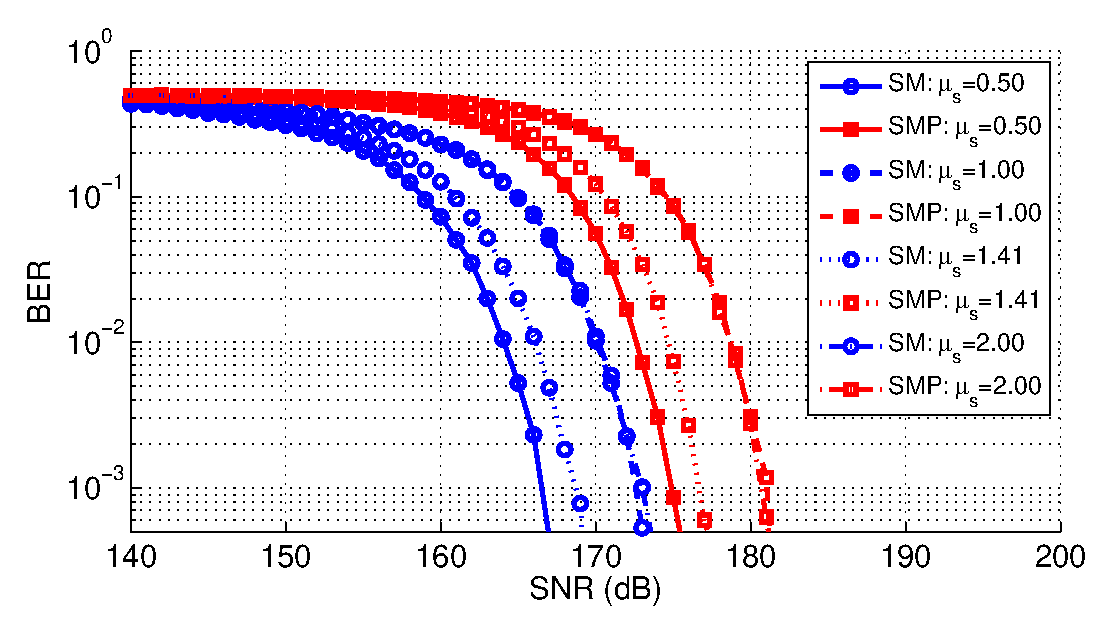
\includegraphics[width=0.9\textwidth]{figMSN4B4.eps}
				\caption{4 bits/sym}
				\label{figMSN4B4}
			\end{subfigure}
			
			\begin{subfigure}{\textwidth}
				\centering
				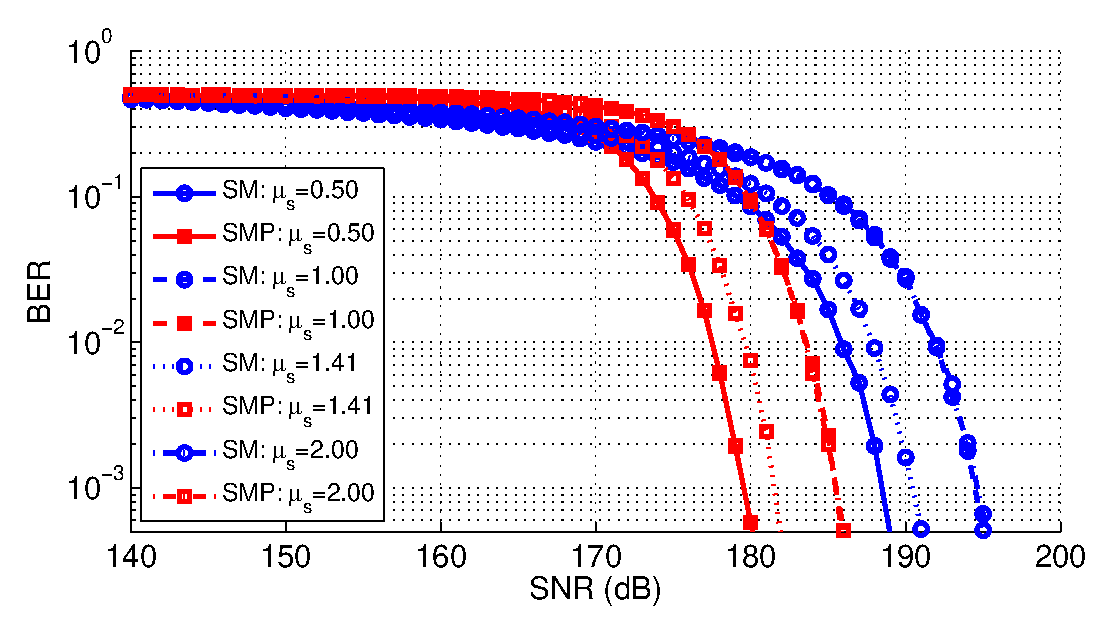
\includegraphics[width=0.9\textwidth]{figMSN4B8.eps}
				\caption{8 bits/sym}
				\label{figMSN4B8}
			\end{subfigure}
			
			\caption{BER vs SNR for different $\mu_{\text{s}}$}
			\label{figMSBvS}
	\end{figure}
	\clearpage% Flush page
%}

In this chapter, we investigated the use of SM and SMP with both imaging and non--imaging receivers in a MIMO VLC system. This effort was achieved via the creation of an analysis framework and normalization approach to enable performance characterization between systems. The results show that an imaging receiver provides significant SNR ($\approx$ 45 dB) gains over non--imaging receiver for SM and SMP in a practical indoor scenario. For lower spectral efficiencies (4 bits/sym), SM performs 8-10 dB better than SMP while at higher spectral efficiencies (8 bits/sym), SMP gives 8-10 dB performance improvement. This is because the imaging receiver helps decorrelate the parallel channel gains as compared to non--imaging receiver. To achieve ideal performance for a given indoor configuration, parameters $\alpha_{\text{s}}$, $\eta_{\text{s}}$ and $\mu_{\text{s}}$ should be carefully selected. From the simulations we can conclude that the imaging MIMO system performs best when a spot is completely enveloped by a single pixel and adjacent spots each lie on adjacent pixels. For the simulation cases considered, $\alpha_{\text{s}}\leq 1$, $\eta_{\text{s}}$ = 0 and $\mu_{\text{s}}$ = 0.5 were found to provide the best system performance.
%\begin{figure}
	%\centering
		%\begin{subfigure}{\textwidth}
			%\caption{}
			%\label{}
		%\end{subfigure}
		%\caption{}
		%\label{}
%\end{figure}